\documentclass[twocolumn,lengthcheck,superscriptaddress]{revtex4-1}

\usepackage{amsmath}
\usepackage{amsthm}
\usepackage{amssymb}
\usepackage{graphicx}
\usepackage{hyperref}
\usepackage{color}
\usepackage{braket}

\newcommand{\tr}{\operatorname{tr}}
\newcommand{\vol}{\operatorname{vol}}
\newcommand{\supp}{\operatorname{supp}}
\newcommand{\dist}{\operatorname{dist}}
\newcommand{\operator}[1]{\ensuremath{\widehat{#1}}}
\newcommand{\ic}{\ensuremath{i}}
\renewcommand{\d}{\ensuremath{d}}
\newcommand{\vx}{\ensuremath{\vec{x}}}
\newcommand{\vk}{\ensuremath{\vec{k}}}

\def\su2{\textsl{SU}(2)}
\def\o3{\textsl{O}(3)}
\def\uone{\textsl{U}(1)}
\def\u2{\textsl{U}(2)}
\def\CL{\textsl{CL}}
\def\CR{\textsl{CR}}
\def\CU{\textsl{CU}}
\def\CAv{\mathbf{Int}}
\def\gl2c{\textsl{GL}(2, \mathbb{C})}
\def\lasu2{\mathfrak{su}(2)}
\def\lauone{\mathfrak{u}(1)}

\newtheorem{theorem}{Theorem}
\newtheorem{proposition}{Proposition}
\newtheorem{lemma}{Lemma}
\newtheorem{corollary}{Corollary}

\theoremstyle{definition}
\newtheorem{definition}{Definition}
\newtheorem{example}{Example}

\theoremstyle{remark}
\newtheorem{remark}{Remark}


\begin{document}

\title{Tensor networks and quantum field theory}

\author{Tobias J.\ Osborne}
\affiliation{Institut f\"ur Theoretische Physik, Leibniz Universit\"at Hannover, Appelstr. 2, 30167 Hannover, Germany}

\begin{abstract}
	Here we describe how tensor network states --- a quantum information theory inspired tool originally arising in the study of quantum spin systems --- can be used to understand the physics of quantum fields. In particular, we review the tensor network formalism and outline its application to the study of ground state physics and scattering amplitudes. We describe two approaches, one based on the Lie-Trotter expansion within the hamiltonian formalism, and a second based on the lagrangian formalism which represents the path integral as a tensor network. We find, exploiting the second approach, that all scattering amplitudes are determined by a special convex set. Our aim in this paper is to present recent developments in condensed matter theory with a quantum field theory audience in mind. 
\end{abstract}

\maketitle

\section{Introduction }
Quantum field theory is now understood as an effective theory describing the large scale low energy physics \cite{wilson:1975a,wilson:1974a}. By exploiting the correspondence between a statistical physics system at criticality and a quantum field Wilson in one fell swoop resolved all the troubling ``infinities'' plaguing quantum field theory. And so it is that quantum field theory has become a tool par excellence in physics; to understand the large-scale effective physics of any system we need only identify the fixed point --- often uniquely defined by the symmetries of the system --- to which it belongs and, often enough, the resulting QFT describing that situation is amenable to perturbation theory allowed us to deploy the apparatus of Feynman diagrams. 

Tensor network papers: \cite{perez-garcia:2006a}\cite{orus:2013a, evenbly:2011a, evenbly:2009a}\cite{verstraete:2004a}
\cite{vidal:2007a}\cite{levin:2007a}\cite{gu:2009a}


Perturbative QFT is useful and powerful but nonperturbative field theory still contains many mysteries: tantalising hints, via holography, of the power of QFT. Complex network of relationships via holographic duality.

The lattice is a good regulator allowing computers to be brought to bear on deep problems. Amazing insights
\cite{wilson:1974b} from confinement to the hadron spectrum \cite{duerr:2008a}.

The lattice 



The path integral is the way to work with QFT


\cite{horava:2008a}\cite{ardonne:2004a}\cite{horava:2009a}\cite{swingle:2012a}\cite{aharonov:2003a}\cite{rudolph:2002a}\cite{ryu:2006a}\cite{ryu:2006b}\cite{nishioka:2009a}\cite{maldacena:2013a}\cite{hartman:2013a}


Here we must cite Swingle, Vidal, Verstraete, Maldacena, Susskind, Takayanagi etc.....

Important points:
\begin{enumerate}
	\item Path integral formalism to calculate $n$-point functions.
	\item Path integral on the lattice = statistical mechanics.
	\item Method 1: trotter
	\item Method 2: Stat. mech. = lifshitz PEPS.
	\item Scattering amplitudes as $n$-point functions.
	\item Removing the cutoff: 2nd (higher) order phase transition; scaling limit.
	\item Variational calculation of $n$-point functions 
	\item Path integrals+perturbation theory: good for weak coupling bad for strong coupling; TNS good for strong coupling bad for weak.
\end{enumerate}


Since their emergence in 1987 in the condensed matter theory literature there has been an amazing amount of progress in the development of tools, both analytic and numeric, for the study of tensor network states. We cannot do proper justice to the literature here, and we only summarise a couple of the highlights. 

In this paper we argue that tensor network methods are reaching a maturity so that they may be profitably employed as an alternative to the path integral in the study of correlated quantum fields. Here  

In this sense tensor-network methods have become a natural alternative to the path integral appropriate for 

The purpose of this letter is to interpret QFT in the language of tensor networks with a view to formalising possible approaches to studying holographic dualities and the calculation of  To this end we describe two natural approaches to studying the statics and dynamics of QFT via TNS, namely, in the hamiltonian setting familiar to condensed matter theory and a second approach by directly representing the full path integral as a TNS. We then argue how to obtain continuum limits and briefly 

\section{What is a tensor network?}

Tensor networks provide an economic framework to parametrise tensors with many indices. Here we provide a brief overview of the tensor network formalism and sketch some calculational techniques. For some recent reviews of this material see, e.g., \cite{orus:2013a, evenbly:2011a, evenbly:2009a}.

\subsection{Tensor diagrams}

We begin our discussion by considering $n$-index tensors: these are, for us, nothing more than collections $\psi$ of $d_1d_2\cdots d_k$ complex numbers $\psi_{j_1j_2\cdots j_n}$, where $j_k = 1, 2, \ldots, d_k$ and  $d_k$ is the dimension of the index. While we sometimes use the ``upstairs'' and ``downstairs'' notation for indices --- basically in order to unclutter our expressions --- this should not be interpreted as implying that the tensor transforms in any particular way under Lorentz transformations (whose action is not even defined here).

A key device we exploit in the following is to visualise an $n$-index tensor $\psi$ as a vertex (really a circle) with $n$ legs, one for each index $j_k$, $k = 1, 2, \ldots, n$:
\begin{center}
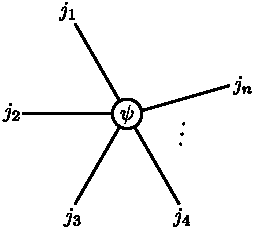
\includegraphics{psitns.pdf}
\end{center}
According to such a visualisation tensors such as vectors are represented as a circle with one leg, matrices as a circle with two legs, and so on:
\begin{center}
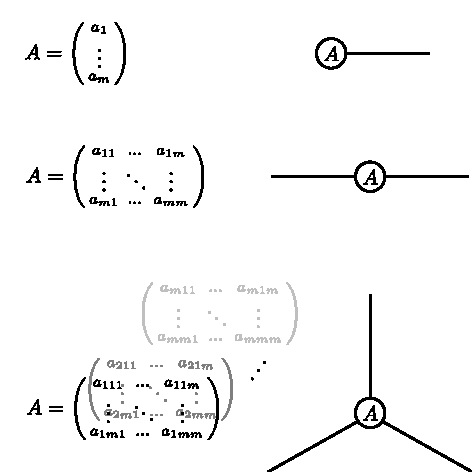
\includegraphics{tns1.pdf}
\end{center}
The contraction of the indices of two tensors is then represented by joining the legs of the corresponding indices. For example:
\begin{center}
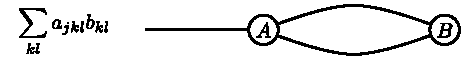
\includegraphics{tns2.pdf}
\end{center}

\subsection{Tensor networks}
A \emph{tensor network} is then the tensor $\psi$ associated with a diagram, actually a \emph{graph} $G$, consisting of a collection of tensors, represented as \emph{vertices}, whose indices are contracted according to the \emph{contraction pattern} described by the edges of the graph. The result is a tensor with a number of indices given by the external or ``dangling legs'' of the diagram. 

The canonical example of a tensor network is the \emph{matrix product state} tensor:
\begin{center}
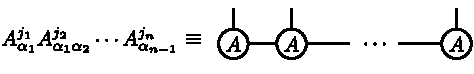
\includegraphics{mps.pdf}
\end{center}

Calculating the value of a tensor network for a given configuration $j_1j_2\cdots j_n$ of the external legs is called \emph{contracting} a tensor network. The problem of contracting, or even approximating the contraction of, an arbitrary tensor network is, in general, \emph{hard}: even \emph{planar} tensor networks can be arbitrarily difficult \cite{schuch:2007a}. Tensor networks are, in general, useful only when they have some additional structure, such as short-ranged correlations (more on this later), topological simplicity, i.e., containing only a few loops, or causal structure, e.g., the tensors are isometries. 


\section{Operations on tensor networks}There are a couple of basic operations one can perform on a tensor network to obtain (sometimes simpler) new networks. The first operation is \emph{partial contraction}: here a collection of vertices and their corresponding tensors are identified and the indices corresponding to all the edges connecting these vertices are contracted. The original tensors are then replaced by the resulting amalgamation: 
\begin{center}
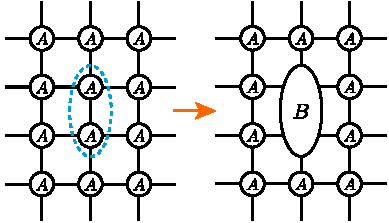
\includegraphics{partialcont.pdf}
\end{center}


The second key primitive is that of \emph{tensor splitting}: here we first collect the external legs of a tensor into two groups which are then regarded as two multi-indices. For example, suppose we have the $n$-index tensor $A$ inside our network: we could collect the first $k$ indices together as the multi index  $\alpha \equiv [j_1j_2 \cdots j_k]$ --- running, say, in lexicographic order through the $d_1d_2\cdots d_k$ assignments of the indices  --- and the remaining indices together as $\beta \equiv [j_{k+1}\cdots j_n]$. This bundling of indices gives us a $2$-index tensor $A_{\alpha\beta}$, where $\alpha$ can be taken to run from $1$ to $d_1\cdots d_k$ and $\beta$ from $1$ to $d_{k+1}\cdots d_n$. We may now regard $A$ as a \emph{matrix}. The tensor splitting operation is then carried out by exploiting the \emph{singular value decomposition} \cite{horn:1990a} to write $A$ as a product of an isometry $U$, a diagonal matrix $d$ with positive entries, and another isometry $V$: 
\begin{equation}\label{eq:svd}
	A = UdV.
\end{equation}
Graphically this is represented as:
\begin{center}
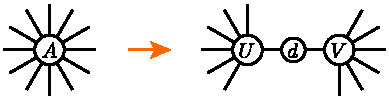
\includegraphics{tensorsplitting.pdf}
\end{center}
Note that the original tensor is replaced with a contraction of three tensors and, in the process, the \emph{degree} of the new vertices in the network is reduced. This procedure may be recursively applied to all the tensors in an arbitrary network to produce a new tensor network with maximal degree bounded above by $3$. (Note: it is impossible, in general, to reduce the degree of all the vertices to $2$ or below via the process.)

The third primitive is \emph{truncation}. Focus on one edge $e$ in a tensor network: this represents a contraction of two specific indices of two tensors. That is, we perform a sum over all the values of the index $\alpha$ indicated by the edge $e$ and shared by the two tensors at the ends of the edge:
\begin{equation}
	\sum_{\alpha = 1}^{d} \cdots A_{\cdots \alpha} B_{\alpha \cdots} \cdots.
\end{equation}
The truncation procedure is an approximation technique where we simply sum over fewer of the possible values of $\alpha$:
\begin{equation}
	\sum_{\alpha = 1}^{d} \cdots A_{\cdots \alpha} B_{\alpha \cdots} \cdots \mapsto \sum_{\alpha = 1}^{d'} \cdots A_{\cdots \alpha} B_{\alpha \cdots} \cdots,
\end{equation}
with $d' < d$. Truncation is particularly effective in combination with tensor splitting: when the diagonal matrix $d$ in Eq.~(\ref{eq:svd}) has many small entries we can simply replace the sum over $\beta$ with a sum over a smaller range, including only the indices corresponding to large entries.

A final approximation operation frequently useful in studying quantum states generated by local dynamics is the \emph{Lie-Trotter} expansion:
\begin{equation}
	e^{A+B} \approx (e^{A/m}e^{B/m})^m,
\end{equation}
where $n$ is a positive integer and $A$ and $B$ are operators on some hilbert space $\mathcal{H}$. This approximation improves as $n$ is increased and becomes an identity in the limit $m\rightarrow \infty$. This result allows us to approximate the propagator $U(t) = e^{-itH}$ --- an $n$-index tensor --- for a quantum spin system with a \emph{local} hamiltonian $H$ by a tensor network involving small-index tensors. To see how this works suppose that $H$ is a hamiltonian for a chain of $n$ quantum spins (similar results hold in higher dimensions):
\begin{equation}
	H = \sum_{j=1}^{n-1} h_j,
\end{equation}
where $h_{j}$ is a local interaction term which acts nontrivially only on spins $j$ and $j+1$. Next collect together the even-numbered (respectively, odd numbered) interactions:
\begin{equation}
	A = \sum_{k=1}^{\lfloor (n-1)/2 \rfloor} h_{2k} \quad \text{and} \quad B = \sum_{k=1}^{\lceil (n-1)/2 \rceil} h_{2k-1}.
\end{equation} 
Now $A$ and $B$ only contain terms which mutually commute with each other, so that $e^{A} = \prod_{k} e^{h_{2k}}$ and $e^{B} = \prod_{k} e^{h_{2k+1}}$. Applying the Lie-Trotter expansion allows us to replace $e^{zH}$ with the product
\begin{equation}
	e^{zH} \approx \left(\prod_{k} e^{\frac{z}{m}h_{2k}}\prod_{k'} e^{\frac{z}{m}h_{2k'}}\right)^m,
\end{equation}
which is a tensor network of $mn$ degree-$4$ tensors. Graphically this is represented by: 
\begin{center}
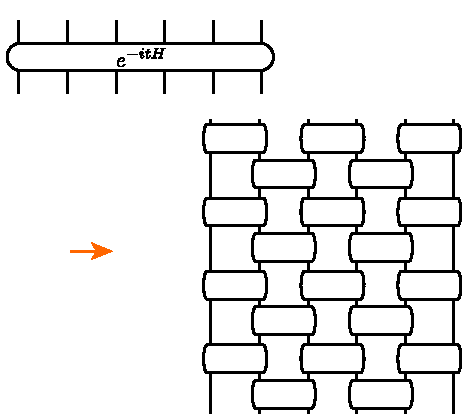
\includegraphics{lietrotter.pdf}
\end{center}
We've thus reduced the contraction of a single degree $2n$ tensor to contracting a network of smaller tensors. In general the difficulty of these two different tasks is roughly equivalent, however, there are cases where the Lie-Trotter network can be exploited to develop useful approximation methods


\section{Tensor network states}
Tensor network states (TNS) are quantum states of a many body quantum system associated with a tensor network. The systems we typically think about are quantum spin systems comprised of $n$ distinguishable quantum spins with local hilbert spaces $\mathcal{H}_j$, $j = 1, 2, \ldots, n$; the total hilbert space is then $\mathcal{H}\cong \bigotimes_{j=1}^{n} \mathcal{H}_j$. It is common to assume that $\mathcal{H}_j$ is finite dimensional, with dimension $d_j$, although there is no fundamental reason preventing everything from straightforwardly applying to infinite dimensional systems. An arbitrary state $|\psi\rangle$ of $\mathcal{H}$ can be written as
\begin{equation}
	|\psi\rangle = \sum_{j_1 = 1}^{d_1}\cdots \sum_{j_{n} = 1}^{d_{n} } \psi_{j_1j_2 \cdots j_{n}}|j_1\rangle \cdots |j_{n}\rangle,
\end{equation} 
where $|j_k\rangle$ is an arbitrary orthonormal basis for $\mathcal{H}_j$. The state $|\psi\rangle$ is encoded in the $d_1d_2\cdots d_n$ components of the $n$-index tensor $\psi_{j_1j_2 \cdots j_{n}}$.  When the dangling legs of a tensor $\psi$ are associated with an orthonormal basis of a quantum spin system we obtain a \emph{tensor network state}.

\subsection{Basic properties of tensor network states}The tensor network formalism exposes some very powerful structural information about quantum states. 

The first property is that a tensor network state is always manifestly a \emph{state}. This is an extremely useful property not shared by other representations (e.g., a truncated perturbation series around some mixed state does not usually determine a positive state).

The second property is that expectation values of (local) operators may be computed by contracting a related tensor network: let $|\psi\rangle$ be a TNS and $M$ some (local) operator on the $l$th spin. Then the expectation value $\langle M \rangle$ is determined by
\begin{equation}
	 \sum_{j_1 = 1}^{d_1}\cdots\sum_{j_l,k_l = 1}^{d_1} \cdots \sum_{j_{n} = 1}^{d_{n} } \psi^*_{j_1j_2 \cdots j_{n}}\psi_{j_1 \cdots j_{l-1}k_l j_{l+1} \cdots j_{n}} M_{j_lk_l},
\end{equation}
which is the contraction of three tensor networks: one for $\psi^*$, one for $M$, and one for $\psi$.
For example, suppose we have a TNS whose coefficients are determined by the network
\begin{center}
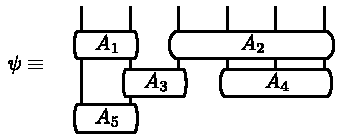
\includegraphics{psinw.pdf}
\end{center}
Then the expectation value of a hermitian operator $M$ on the 3rd spin is given by the contraction
\begin{center}
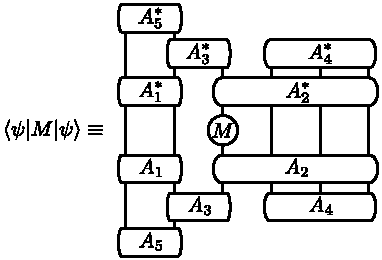
\includegraphics{expvals.pdf}
\end{center}
Closely related to the calculation of expectation values is the construction of the \emph{reduced density operator}. Let $|\psi\rangle$ be a tensor network state. Form the corresponding density operator $\rho \equiv |\psi\rangle\langle \psi|$: this is a tensor network with twice the number of external legs and every tensor doubled. Take the partial trace over all spins outside of region $A$; this operation is found by connecting the indices corresponding to the legs in the complement in $A$ as follows:
\begin{center} 
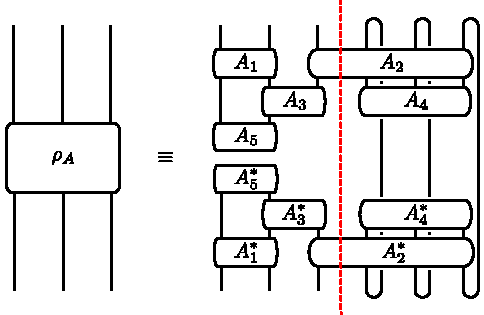
\includegraphics{ptrace.pdf}
\end{center}

The third remarkable property is that we obtain an upper bound on the entropy of entanglement associated a region $\mathcal{R}$ in the network. This result may be argued as follows.  

\section{Tensor networks from hamiltonians}\hspace{-1em}
In this section we'll discuss a now-standard way to obtaining a tensor network state representation of the ground state and low-lying excitations of a complex quantum system. As we'll discuss, in the quantum field setting there are additional complications arising when removing (lattice) regulator. The discussion here is framed in the \emph{hamiltonian} setting: our input is the regulated \emph{quantum} hamiltonian for the system. We use as regulator the spatial lattice $L_a \equiv a\mathbb{Z}^D\subset \mathbb{R}^D$, with lattice spacing $a$. The discussion throughout this paper is illustrated in terms of the running example of $\phi^4$ theory; additional fields and fermions do not present any new major conceptual difficulties (beyond fermion doubling). To further simplify our discussion in this section we only consider this model in $(1+1)$ dimensions (the extension to higher dimensions is only sketched). 

The hamiltonian of $\phi^4$ theory on a lattice with lattice spacing $a$ is expressible as 
\begin{equation}
	H_a = a\sum_{j\in L_a} \frac{\widehat{p}_j}{2a^{2}} + \frac{(\widehat{x}_j-\widehat{x}_{j+1})^2}{2a^2} + \frac{\mu_0^2}{2} \widehat{x}_j^2 + \frac{\lambda}{4!} \widehat{x}_j^4,
\end{equation}
where $[\widehat{x}_j, \widehat{p}_k] = i\delta_{jk}$. To a tensor-network practitioner the most natural way to approach the approximation of the ground state is to first make a guess $|\Phi_0\rangle$ for the ground state as a simple tensor network state and then to improve this guess. One tried and true approach to doing this is to use \emph{mean-field theory} to obtain $|\Phi_0\rangle$ as a trivial matrix product state and then to simulate its \emph{imaginary time evolution} 
\begin{equation}
	|\Phi(\beta)\rangle \equiv \frac{e^{-\beta H_a}|\Phi_0\rangle}{\|e^{-\beta H_a}|\Phi_0\rangle\|}.
\end{equation}
If $H$ has a spectral gap and if the initial condition $|\Phi(0)\rangle \equiv |\Phi_0\rangle$ has some overlap with the true ground state $|\Omega\rangle$, i.e., $\langle \Phi(0)|\Omega\rangle \not= 0$, then we obtain an exponentially improving approximation $|\Omega(\beta)\rangle$ to $|\Omega\rangle$.
As we saw in the previous section, the Lie-Trotter expansion can be utilised to approximate $e^{-\beta H_a}$  with a tensor network. When this tensor network is contracted against the tensor network for a product state we obtain a matrix product state $|\Psi\rangle$ with bond dimension equal to $\text{const.}^{\text{\# of layers}}$:


\section{Tensor networks from path integrals}
In this section we describe how to construct a special quantum state, the \emph{quantum Lifschitz state}, which encodes all of the $n$-particle scattering amplitudes for a given quantum (field) theory. This idea traces its origin back at least to the work of Rudolph and Ta-Shma and Aharonov \cite{rudolph:2002a, aharonov:2003a} and has found recent applications by Ardonne in condensed matter theory where it is known as a \emph{quantum Lifschitz theory} \cite{ardonne:2004a}, and later in the study of quantum gravity by Ho\v{r}ava \cite{horava:2009a,horava:2008a}. In contrast to the aforementioned applications in condensed matter theory and quantum gravity we are not proposing new exactly solvable theories, rather, we exploit the quantum Lifschitz construction to encode the full path integral as a pure quantum state which we then subsequently represent as a tensor network. It is worth noting that, in the context of constructive quantum field theory, the quantum Lifschitz state is an encoding of all the \emph{Schwinger functions} of the theory.  

The basic input to any calculation in QFT is the lagrangian $\mathcal{L}$. To keep a concrete example in mind think of $\phi^4$ theory in $D+1$ dimensions:
\begin{equation}
	\mathcal{L} = \frac12 (\partial_\mu\phi)^2 - \frac12m^2 \phi^2 -\frac{\lambda}{4!}\phi^4,
\end{equation}
however, everything we discuss here is valid in generality (in particular, everything we say here will apply equally to relativistic and nonrelativistic settings).  Using the lagrangian we can calculate any $n$-point correlation function using the path integral according to the standard formula
\begin{multline}	
	\langle  T[\phi(x_1)\cdots \phi(x_n)] \rangle\equiv\\ \lim_{T\rightarrow \infty(1-i\epsilon)} \frac{\int \mathcal{D}\phi \, \phi(x_1)\cdots \phi(x_n)e^{i\int_{-T}^T d^4x\, \mathcal{L}}}{\int \mathcal{D}\phi\, e^{i\int_{-T}^T d^4x\, \mathcal{L}}}.
\end{multline} 
Before such a path integral can be evaluated --- or even approximated --- it is generally necessary to \emph{regulate} the theory by applying a cutoff $\Lambda$. Now, in the context of tensor networks and quantum information, the most natural regulator is the lattice, with lattice spacing $a = \frac{1}{\Lambda}$, and we don't hesitate to use it throughout. In this way we discretise our continuous field(s) $\phi(x)$ onto the integer lattice $a\mathbb{Z}^{D+1}$; we restrict our coordinates to lattice points $x = an$, $n \in \mathbb{Z}^{D+1}$. Write the field evaluated at lattice points as $\phi_{n} = \phi(x)$; thus we discretise derivatives as $\partial_\mu \phi(x) \mapsto (\phi_{n + e_{\mu}} - \phi_{n})/a$,   where $e_\mu$ is the unit lattice vector in the direction $\mu$. Thus our potentially ill-defined path integral is replaced, after discretisation, by the better-behaved iterated integral
\begin{equation}
	\int \mathcal{D}\phi \mapsto \int [d\phi] \equiv \int \left(\prod_{n\in\mathbb{Z}^{D+1}} d\phi_n \right).
\end{equation}
A further important device that we also initially exploit is to make a Wick rotation of time $t\mapsto -i\beta$: this turns our path integral expression for the correlation functions into a statistical mechanical problem:
\begin{equation}\label{eq:wrcorr}
	\langle  \phi(x_{1})\cdots \phi(x_n) \rangle\equiv \frac{1}{\mathcal{Z}}\int [d\phi] \, \phi_{m_1}\cdots \phi_{m_n} e^{-S},
\end{equation} 
where $x_1 = a m_1, x_2 = a m_2, \ldots, x_1 = a m_n$, $\mathcal{Z} = \int [d\phi] \, e^{-S}$ and, e.g., $S = a^{D+1}\big(\sum_{\langle m,n\rangle\in \mathbb{Z}^{D+1}} (\phi_m-\phi_n)^2/(2a^2) + \sum_{n} m^2\phi_n^2/2 + \lambda \phi_n^4/4!\big)$.


To practitioners in tensor networks an expression such as Eq.~(\ref{eq:wrcorr}) is rather suggestive. This is because we can introduce a special pure quantum state $|\Phi\rangle$, which we call the \emph{quantum Lifschitz state}, encoding all the information we can extract from a partition function. To explain this construction suppose we have a classical system which can be in one of $N$ different configurations, $x = 1, 2, \ldots, N$. (One example to keep in mind is the classical Ising model on an $L\times L$ lattice, here $x$ runs over all the configurations, labelled in lexicographic order from $1$ to $2^{L^2}$, of the spins.) Write the hamiltonian as $H = \sum_{x=1}^N E_j(x) |x\rangle\langle x|$, where we exploit quantum notation for classical systems: they are, for us, simply systems diagonal in a given ``position'' basis. The thermal state for the system is simply $\rho = e^{-\beta H}/\mathcal{Z}$. The trick is now to take the square root of the probabilities $p(x) = e^{-\beta E(x)}/\mathcal{Z}$ \cite{rudolph:2002a, aharonov:2003a} and build the \emph{pure} quantum state 
\begin{equation}
|\Phi\rangle \equiv \frac{1}{\sqrt{\mathcal{Z}}}\sum_{x=1}^N e^{-\frac12\beta E(x)}|x\rangle,
\end{equation}
where $|x\rangle$ is an orthonormal basis corresponding to the $N$ possible configurations of the classical system. The state $|\Phi\rangle$ encodes the expectation value of any observable. To see this suppose $O:\{1,2,\ldots, N\}\rightarrow \mathbb{C}$ is an observable for the classical system (e.g., a multi-point correlation function such as $\sigma_{j_1}\sigma_{j_2}\cdots \sigma_{j_N}$). We can build a quantum observable which gives us the same expectation values:
\begin{equation}
	\widehat{O} \equiv \sum_{x=1}^N O(x) |x\rangle\langle x|.
\end{equation}
We hence obtain 
\begin{equation}
\langle \Phi|\widehat{O}|\Phi\rangle = \langle O\rangle \equiv \frac{1}{\mathcal{Z}}\sum_{x=1}^N O(x) e^{-\beta E(x)}. 
\end{equation}

This construction is easily extended to encode imaginary time path integrals. As long as the action is real valued the above construction goes through unmodified: when we apply the procedure described here to a Wick-rotated path integral we obtain the following state of a lattice of a $(D+1)$-dimensional spatial lattice of harmonic oscillators 
\begin{equation}\label{eq:qls}
	|\Phi\rangle \equiv \frac{1}{\mathcal{Z}}\int [d\phi] \,e^{-\frac{1}{2}S[\phi]}  |\boldsymbol{\phi}\rangle,
\end{equation}
where
\begin{equation}
	|\boldsymbol{\phi}\rangle \equiv \bigotimes_{x\in a\mathbb{Z}^{D+1}} |\phi(x)\rangle,
\end{equation}
and $|\phi(x)\rangle$ is an improper \emph{position eigenstate} of the harmonic oscillator for site $x$ localised at the harmonic oscillator position $\phi(x)$. We can obtain this state by applying the (exponential of the) operator 
\begin{equation}
	\widehat{S} \equiv \frac{a^{D-1}}{2}\sum_{\langle m,n\rangle} (\widehat{\phi}_m-\widehat{\phi}_n)^2 + a^{D+1}\sum_{n} \frac{m^2}{2}\widehat{\phi}_n^2 + \frac{\lambda}{4!} \widehat{\phi}_n^4,
\end{equation}
with 
\begin{equation}
	\widehat{\phi}_n  \equiv \phi(an)|\boldsymbol{\phi}\rangle,
\end{equation}
to the \emph{momentum-zero} state
\begin{equation}
	|\Omega\rangle \equiv \bigotimes_{x\in a\mathbb{Z}^{D+1}} |\omega\rangle,
\end{equation}
where
\begin{equation}
	|\omega\rangle \text{``$\equiv$''} \int d\phi\, |\phi\rangle,
\end{equation}
is the improper momentum eigenstate. That is, we have that
\begin{equation}
	|\Phi\rangle \propto e^{-\frac12 \widehat{S}}|\Omega\rangle. 
\end{equation}


One might wonder whether this construction can be extended to deal with the case of arbitrary path integrals. The naive answer is obviously no: if we just take the square roots of the integrand $e^{iS}$ in a path integral then the resulting state $|\Phi\rangle$, constructed as above, has the unfortunate property that $\langle \Phi| \widehat{O}|\Phi\rangle$ is independent of $|\Phi\rangle$! However if we are willing to introduce an ancillary quantum spin we can make an analogous construction. Suppose we have a path integral expression of the form 
\begin{equation}
	\langle O \rangle = \frac{\sum_{x=1}^N O(x) e^{iS(x)}}{\sum_{x=1}^N e^{iS(x)}},
\end{equation}
where $S$ is the action and $O$ an observable. We can again construct a pure quantum state encoding all the information about arbitrary observables $O$ as follows:
\begin{equation}\label{eq:pipurestate}
	|\Phi\rangle = \frac{1}{\sqrt{2\mathcal{Z_+}}}\sum_{x=1}^N e^{\frac{i}{2}S(x)} |x\rangle|0\rangle + \frac{1}{\sqrt{2\mathcal{Z_-}}}\sum_{x=1}^N e^{-\frac{i}{2}S(x)} |x\rangle|1\rangle,
\end{equation}
where
\begin{equation}
	\mathcal{Z_\pm} = \sum_{x=1}^N e^{\pm iS(x)}.
\end{equation}
It is now possible to generalise the construction above to construct quantum operators $\widehat{O}$ whose expectation values give those of their corresponding classical counterparts $O$:
\begin{equation}
	\widehat{O} \equiv 2\sum_{x=1}^N O(x) |x\rangle\langle x|\otimes |1\rangle\langle 0|.
\end{equation}
The auxiliary spin here is thought of as indicating the arrow of time.

The pure states Eq.~(\ref{eq:qls}) and Eq.~(\ref{eq:pipurestate}) are perfect for approximation via tensor network states. However, the state Eq.~(\ref{eq:pipurestate}) does not lend itself so directly to the conclusions of the next section. This can be repaired by introducing one auxiliary quantum spin per edge of the lattice to indicate the arrow of time for each edge, but the resulting construction is somewhat unwieldy. We prefer, instead, to focus on the quantum Lifschitz state Eq.~(\ref{eq:qls}) and deduce statements about the real-time path integral via Wick rotation. (I.e., in the language of constructive quantum field theory we will study the Schwinger functions instead of the Wightman functions.)

Indeed, we will go further: the principle contribution of this project is to promote tensor networks of the form Eq.~(\ref{eq:pipurestate}) to the status of a \emph{definition} for a class of path integrals. The justification of this idea will take us on a long journey.




\section{Parent hamiltonians and convex sets}

\subsection{Parent hamiltonians}
Remarkably, we can also realise $|\Phi\rangle$ as the \emph{ground state} of a natural hamiltonian \cite{ardonne:2004a, verstraete:2006a, perez-garcia:2008a, horava:2008a}. The key to this construction is to introduce a reversible markov chain $M$ which has $p_x \equiv  e^{-E(x)}/\mathcal{Z}$ as its stationary distribution \cite{norris:1997a}, i.e., $\sum_{x=1}^N p_xM_{xy} = p_y$, $\forall y$. Reversibility is the condition that $p_x M_{xy} = p_yM_{yx}$, $\forall x,y$. This motivates us to introduce the  matrix $K$ with matrix elements:
\begin{equation}
	K_{xy} \equiv \sqrt{p_x} M_{xy} \frac{1}{\sqrt{p_y}}.
\end{equation}
Because of the reversibility condition we find that $K$ is real and symmetric, i.e., hermitian. Further, we have that operator $\widehat{K} \equiv  \sum_{x,y=1}^N K_{xy}|y\rangle \langle x|$ has $|\Phi\rangle$ as an eigenvector corresponding to its largest eigenvalue. We obtain our desired hamiltonian by writing $\widehat{H} \equiv \mathbb{I} - \widehat{K}$, this operator has $|\Phi\rangle$ as a ground state with eigenvalue $0$.

Given a probability distribution of exponential form, i.e., $p_x \equiv  e^{-E(x)}/\mathcal{Z}$, $x=1, 2, \ldots, N$, there is a special reversible Markov chain having $p_j$ as its stationary distribution, namely, the Metropolis algorithm \cite{metropolis:1953a}. 
\begin{equation}
	M_{xy} \equiv P(y|x),
\end{equation}
where
\begin{equation}
	P(y|x) \equiv \begin{cases} 1 - \sum_{y\not = x} p(y|x) &\quad y=x \\
	p(y|x) &\quad y \not= x,\end{cases}
\end{equation}
with
\begin{equation}
	p(y|x) \equiv  \min\left\{f(y|x), f(x|y)e^{-\beta (E(y)-E(x))}\right\},
\end{equation}
and we've introduced a \emph{flip process} with transition probabilities $f(y|x)$ inducing transitions between the states of the system.

We now make a judicious choice of flip process to arrive at a \emph{local hamiltonian} having the quantum lifschitz state $|\Phi\rangle$ in Eq.~(\ref{eq:qls}) as its ground state. 

Suppose that 
\begin{equation}
	F_{x} = \int [d\phi d\phi']\, f_x(\phi'|\phi) |\phi'\rangle\langle \phi|,
\end{equation}
$x \in a\mathbb{Z}^{D+1}$ is a \emph{local flip operator}, i.e., an operator whose support is restricted to site $x$: $\supp(F_x) = \{x\}$. This means that the flip probability $f_x(\phi'|\phi)$ is zero if $\phi$ and $\phi'$ differ on any site $y\not=x$, i.e., $f_x(\phi'|\phi)$ can only be nonzero if $\phi$ and $\phi'$ differ \emph{at most} on site $x$.

We then claim that the operator $\widehat{K}_x$ resulting from the above construction has support $\supp(\widehat{K}_x) \subset \{x,x  \pm ae_{1}, x \pm ae_{2}, \ldots, x  \pm ae_{D+1}\}$. This follows from noting, first, that 
\begin{equation}
	p(\phi'|\phi) \equiv  \min\left\{f_x(\phi'|\phi), f_x(\phi'|\phi)e^{- \frac12 (S(\phi')-S(\phi))}\right\}
\end{equation}
inherits a locality property from $f_x(\phi'|\phi)$: it depends on, at most, the values of the configurations $\phi_y$ in a neighbourhood of sites of (lattice) radius $1$ around $x$, i.e., on those sites $y$ with $d(x,y) \le 1$. Thus we deduce that the transition probabilities $P_x(\phi'|\phi)$ arising from $p_x(\phi'|\phi)$ yield a markov matrix $M$ with $\supp(M) \subset \{x,x  \pm ae_{1}, x \pm ae_{2}, \ldots, x  \pm ae_{D+1}\}$.

An alternative construction of a parent hamiltonian follows from the observation that $e^{\frac12 \widehat{S}}|\Phi\rangle \propto |\Omega\rangle$. We use the fact that we can easily construct a local parent hamiltonian for the momentum state $|\Omega\rangle$, e.g., 
\begin{equation}
	\widehat{\pi}_n^2, \quad n\in \mathbb{Z}^{D+1},
\end{equation}
does a good job, to construct the local operator
\begin{equation}
	\widehat{k}_n \equiv e^{-\frac12\widehat{S}} (\widehat{\pi}_n^2) e^{\frac12\widehat{S}}.
\end{equation}	
Using the nonhermitian operator $\widehat{k}_n$ we then obtain a local parent hamiltonian via, e.g.,
\begin{equation}
	\widehat{H} \equiv \sum_{n} |\widehat{k}_n|,
\end{equation}
where $|M| \equiv \sqrt{M^\dag M}$. 

\subsection{The space of reduced density operators}
The ground states of local hamiltonians are extremal objects with a remarkable and deep structure that we are only now beginning to uncover. In this subsection we apply some of the insights obtained in quantum-information inspired studies of the ground-state physics of many particle systems to deduce some striking observations concerning the quantum Lifschitz state and the structure of scattering amplitudes. 

A simple argument \cite{verstraete:2005a}, somewhat analogous to the Kohn-Sham theorem \cite{hohenberg:1964a,kohn:1965a}, exposes an intriguing connection between the correlations of ground states of local  hamiltonians and the geometric properties of a \emph{universal} convex set. We summarise the argument for a chain of quantum spins (spin-$1/2$ degrees of freedom). Write $\mathcal{C}_{\text{TI}}$ for the \emph{convex} set of \emph{all} translation-invariant (both pure and mixed) states of the chain. Suppose that $H = \sum_{j\in\mathbb{Z}} h_{j,j+1}$ is a local hamiltonian for the chain, where $h_{j,j+1}$ acts nontrivially on only pairs of spins $\{j,j+1\}$. We immediately deduce that the energy density $\langle e \rangle$ of $H$ for some state $\omega\in \mathcal{C}_{\text{TI}}$ is a function only of the two-site reduced density operator, i.e., 
\begin{equation}
	\langle e \rangle = \tr(\rho_{01} h_{0,1}),
\end{equation}
where $\rho_{01} \equiv \tr_{\widehat{01}}(\omega)$ is the reduced density operator for sites $01$. Write $\mathcal{C}_{\text{TI}}(0,1)$ for the compact convex $15$-dimensional set of all such two-particle reduced density operators. Because of the constraints of positivity and translation invariance this set is \emph{not} the same as the set of all two-spin density operators.

The simple observation that the energy density of a state $\omega\in \mathcal{C}_{\text{TI}}$ is a linear function only of the two-site reduced density operator has a remarkable consequence: we can reduce the infinite-dimensional minimisation problem for the ground state of $H$ to a \emph{finite-dimensional} minimisation problem over the set $\mathcal{C}_{\text{TI}}(0,1)$, i.e.,
\begin{equation}
	\inf_{\omega\in \mathcal{C}_{\text{TI}}} \langle e \rangle = \min_{\rho_{01}\in \mathcal{C}_{\text{TI}}(0,1)} \tr(\rho_{01} h_{0,1}).
\end{equation}
An analogous argument applies to higher-dimensional lattices.

Thus if we could only obtain a compact geometric characterisation of the set $\mathcal{C}_{\text{TI}}(0,1)$ we'd be able to reduce the study of ground-state problems for local hamiltonians to a finite-dimensional computation. This task is deeply nontrivial. Indeed it is not really expected to ever be completed because a compact efficient characterisation of $\mathcal{C}_{\text{TI}}(0,1)$ would have dramatic consequences for computational complexity: it turns out that for sufficiently high-dimensional spins the task of computing the ground-state energy of a (somewhat baroque) translation-invariant spin chain is a computationally hard problem. 

The set $\mathcal{C}_{\text{TI}}(0,1)$ can be approximated in a variety of ways: inner approximations can be easily obtained using a variational ansatz arising from, e.g., mean-field theory. Outer approximations may obtained by relaxing the infinite number of constraints arising from the joint requirements of translation invariance and positivity. 

We now exploit the above observations to argue that the scattering amplitudes for an arbitrary $D+1$ dimensional local quantum field theory are completely determined by the convex set. 

\section{Quantum gauge theory}
In this section we extend the discussion of the previous sections to cover the case of gauge theory. The ideas here exploit the tensor network representation for the gauge-invariant sector developed in the open science project ``Lattice-gauge-theory-and-tensor-networks'' to produce the quantum Lifschitz state for the gauge-unfixed lattice path integral.

To discuss the construction of a lifshitz state for quantum gauge theory we need to specify our local degrees of freedom: the \emph{local position} degree of freedom is an element of a compact group $G$. The position basis for such a degree of freedom is written as  
\begin{equation}
	|U\rangle, \quad U\in G,
\end{equation}
with inner product
\begin{equation}
	\langle U|V\rangle = \delta(U-V).
\end{equation}
Associated with this space is the hilbert space $L^2(G)$ of square integrable functions on a compact lie group $G$ whose elements may be represented as
\begin{equation}
	|\psi\rangle = \int dU\, \psi(U)|U\rangle,
\end{equation}
where $dU$ is the Haar measure. 

To build the quantum lifschitz state we require a $(D+1)$-dimensional lattice of these local degrees of freedom, which are then associated with the directed links of the lattice.

The two choices $G=\uone$ and $G=\su2$ exemplify the key differences; the more general case does not require the introduction of many new ideas. 

Our objective here is to realise the path integral for lattice gauge theory via the quantum Lifschitz state proposal. To this end we first need to identify the initial fiducial state analogous to the momentum-zero state $|\Omega\rangle$. This state is naturally given as tensor produce over the links of the zero-energy eigenstate $|\omega\rangle$ of the local kinetic-energy operator, 
\begin{equation}
	|\omega\rangle = \int dU \,|U\rangle.
\end{equation}
Using this state we can build the quantum Lifschitz state for an arbitrary nonabelian gauge theory on the lattice by applying the operator 
\begin{equation}
	e^{-\frac12\widehat{S}},
\end{equation}
where
\begin{equation}
	\widehat{S} = \sum_{e\in E} \widehat{u}_e + 
\end{equation}

\section{The continuum limit}
The objective this section we combine the techniques developed in both the open science projects ``Lattice-gauge-theory-and-tensor-networks'' and ``Continuous-Limits-of-Quantum-Lattice-Systems'' to produce a quantum Lifschitz for a full quantum gauge theory.

\section{Conclusions}


\bibliography{tnspi}

\widetext
\appendix
\section{Parent hamiltonians for the Lifschitz state}\label{app:metro}
In this appendix we write out some of the calculations involved in constructing a parent hamiltonian for the Lifschitz state.

\subsection{The Metropolis algorithm}
The Metropolis algorithm is a markov chain which has the gibbs distribution for a classical hamiltonian of the form $H = \sum_{x=1}^N E(x)|x\rangle\langle x|$ as its stationary distribution. To build the markov matrix for this chain we introduce a \emph{flip process} with transition probabilities $f(y|x)$ which induces transitions between the states of the chain. The transition probabilities of the markov chain are now given by
\begin{equation}
	P(y|x) \equiv \begin{cases} 1 - \sum_{y\not = x} p(y|x) &\quad y=x \\
	p(y|x) &\quad y \not= x,\end{cases}
\end{equation}
where
\begin{equation}
	p(y|x) \equiv  \min\left\{f(y|x), f(x|y)e^{-\beta (E(y)-E(x))}\right\}.
\end{equation}
We now check that this markov chain indeed has the gibbs distribution as its fixed point:
\begin{equation}
	\begin{split}
		\sum_{x = 1}^N P(y|x) e^{-\beta E(x)} &= \left(1 - \sum_{z\not = y} p(z|y)\right) e^{-\beta E(y)} + \sum_{x \not= y} p(y|x) e^{-\beta E(x)} \\
		&= \left(1 - \sum_{z\not = y} p(z|y)\right) e^{-\beta E(y)} + \sum_{x \not= y} e^{-\beta E(x)}\min\left\{f(y|x), f(x|y)e^{-\beta (E(y)-E(x))}\right\} \\
		&= \left(1 - \sum_{z\not = y} p(z|y)\right) e^{-\beta E(y)} + \sum_{x \not= y} \min\left\{f(y|x)e^{-\beta E(x)}, f(x|y)e^{-\beta E(y)}\right\} \\
		&= e^{-\beta E(y)} - \sum_{x\not = y} \min\left\{f(x|y)e^{-\beta E(y)}, f(y|x)e^{-\beta E(x)}\right\}  + \sum_{x \not= y} \min\left\{f(y|x)e^{-\beta E(x)}, f(x|y)e^{-\beta E(y)}\right\} \\
		&= e^{-\beta E(y)}.
 	\end{split}
\end{equation}
The markov matrix for the Metropolis algorithm has matrix elements
\begin{equation}
	M_{xy} \equiv P(y|x).
\end{equation}

\subsection{Parent hamiltonians via the Metropolis hamiltonian}
The Lifschitz state for $H$ is given by
\begin{equation}
	|\Phi\rangle \equiv \sum_{x=1}^N e^{-\frac12E(x)}|x\rangle/\sqrt{\mathcal{Z}}.
\end{equation}
(We assume that the eigenvalues $E(x)$ of $H$ are arranged in increasing order.)

Using the markov matrix $M$ for the Metropolis algorithm we build the $K$ operator
\begin{equation}
	\widehat{K} \equiv \sum_{x,y=1}^N e^{-\frac{\beta}{2}(E(x)-E(y))} P(y|x) |y\rangle\langle x|.
\end{equation}


\subsection{Parent hamiltonians via generalised Metropolis operators}
In this subsection we describe an alternative procedure to directly construct parent hamiltonians. The idea here is to exploit the representation of the Lifschitz state as
\begin{equation}
	|\phi\rangle \propto e^{-\frac{\beta}{2} H}|+\rangle,
\end{equation}
where
\begin{equation}
	|+\rangle \equiv \sum_{x=1}^N |x\rangle.
\end{equation}
Now it is easy to find operators which annihilate $|+\rangle$, e.g., just choose
\begin{equation}
	P \equiv \mathbb{I} - |+\rangle\langle+|.
\end{equation}
Using such an operator we can easily build a positive hermitian operator annihilating $|\Phi\rangle$:
\begin{equation}
	\widehat{K} \equiv  \left(e^{-\frac{\beta}{2} H} P e^{\frac{\beta}{2} H} \right)^\dag\left(e^{-\frac{\beta}{2} H} P e^{\frac{\beta}{2} H} \right).
\end{equation}

\end{document}


